\documentclass{article}
\usepackage[dvipsnames]{xcolor}

\makeatletter
\makeatother

\usepackage{tikz,pgflibraryshapes,amsmath}
\usetikzlibrary{arrows, calc, decorations.pathmorphing,plotmarks}

\usepackage[psfixbb,graphics,tightpage,active]{preview}

\PreviewEnvironment{tikzpicture}
\newlength{\imagewidth}
\newlength{\imagescale}

\begin{document}

\usetikzlibrary{calc,arrows}
% Domain Variables 
\pgfmathsetmacro\lx{16};
\pgfmathsetmacro\ly{9};

\pgfmathsetmacro\xmin{0};
\pgfmathsetmacro\xmax{\lx};
\pgfmathsetmacro\ymin{0};
\pgfmathsetmacro\ymax{\ly};

\pgfmathsetmacro\pDx{0.75};
\pgfmathsetmacro\pDxOffset{0.03};
\pgfmathsetmacro\pDy{0.42};
\pgfmathsetmacro\pDyOffset{0.08};

% colors

% style
\tikzset{NNBox/.style={draw,color=OliveGreen,line width=2pt, fill=OliveGreen!10!white}}
\tikzset{PBox/.style={draw,color=Orange,line width=2pt, fill=YellowOrange!20!white}}
\tikzset{DBox/.style={draw,color=NavyBlue,line width=2pt}}
\tikzset{SDBox1/.style={fill,color=Black!30!white,line width=-1pt}}
\tikzset{SDBox2/.style={fill,color=Black!15!white,line width=-1pt}}
\tikzset{SDBox3/.style={fill,color=Black!5!white,line width=-1pt}}
\tikzset{empty/.style={inner sep=0,outer sep=0}}

\tikzset{boundary/.style={draw,color=black,line width=2pt}}
\tikzset{levelset/.style={draw,color=blue,line width=2pt}}
\tikzset{axis/.style={line width=1, fill=gray, draw=gray,-triangle 45,postaction={draw, line width=1, shorten >=7, -}}}
\tikzset{arrow/.style={draw, line width=1.5, shorten >=6pt, shorten <=6pt, ->}}
\tikzset{icefront/.style={draw,color=red,line width=2pt}}

\newpage
\begin{center}
\begin{tikzpicture}
    % Coordinate
    \coordinate (Nll) at (\xmin,\ymin+\pDy*\ly+\pDyOffset*\ly);
    \coordinate (Ntr) at (\xmax, \ymax);
    \coordinate (Dll) at (\xmin,\ymin);
    \coordinate (Dtr) at (\xmin+\pDx*\lx, \ymin+\pDy*\ly);
    \coordinate (Pll) at (\xmin+\pDx*\lx+\pDxOffset*\lx,\ymin);
    \coordinate (Ptr) at (\xmax, \ymin+\pDy*\ly);
    
    \coordinate (SD1ll) at ($(Dll)+(0*\lx,0)$);
    \coordinate (SD1tr) at ($(SD1ll)+(0.27*\lx,  \pDy*\ly)$);
    \coordinate (SD2ll) at ($(SD1tr)+(0,        -\pDy*\ly)$);
    \coordinate (SD2tr) at ($(SD2ll)+(0.24*\lx,  \pDy*\ly)$);
    \coordinate (SD3ll) at ($(SD2tr)+(0,        -\pDy*\ly)$);
    
    % ============================== Neural network ==============================
    \draw[NNBox] (Nll) rectangle (Ntr);
    \node[empty] (figNN) at ($(Nll)!0.5!(Ntr)+(-0.22*\lx, -0.03*\ly)$) 
    {\includegraphics[width=0.65\textwidth]{NNs.pdf}};
    % text
	 \Large
    \node[empty, color=OliveGreen, scale=1] (NNtext) at ($(figNN)+(0,0.24*\ly)$) {Neural Network};
	 \large
    \node[empty, color=OliveGreen, scale=0.8] (update) at ($(figNN)+(0.35*\lx,0.24*\ly)$) {Update the weights};
    \node[empty, color=OliveGreen, scale=0.8] (Optimization) at ($(figNN)+(0.64*\lx,0.1*\ly)$) {Optimization};
    \node[empty, color=OliveGreen, scale=0.8] (Loss) at ($(figNN)+(0.4*\lx,0.06*\ly)$) {Loss Function};
    % Equations
	 \large
    \node[empty] (Lossmath) at ($(figNN)+(0.4*\lx,0*\ly)$) {$\mathcal{L}=\mathcal{L}_u+\mathcal{L}_g+\mathcal{L}_C+\mathcal{L}_f$};
    \node[empty, yscale=8] (case) at ($(figNN)+(0.25*\lx,0*\ly)$) {$\}$};
    % arrows
    \draw[arrow, color=OliveGreen,  to path={-| (\tikztotarget)}] (Lossmath) edge (Optimization) ;
    \draw[arrow, color=OliveGreen,  to path={|- (\tikztotarget)}] (Optimization) edge (update);
    \draw[arrow, color=OliveGreen] (update) -- (NNtext);

    % ============================== Data ==============================
    \draw[SDBox1] (SD1ll) rectangle (SD1tr);
    \draw[SDBox2] (SD2ll) rectangle (SD2tr);
    \draw[SDBox3] (SD3ll) rectangle (Dtr);
    \draw[DBox] (Dll) rectangle (Dtr);
    % Embedded Figures
    \node[empty] (fig1) at ($(SD1ll)!0.5!(SD1tr)+(0.015*\lx, 0.05*\ly)$)
	 {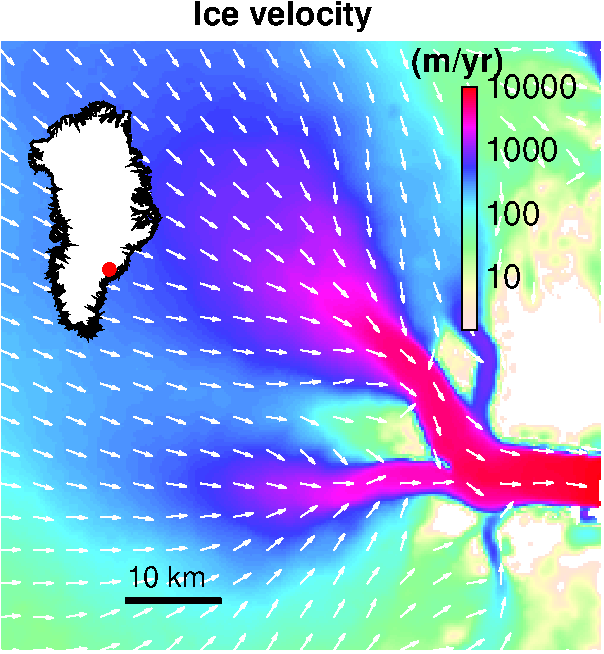
\includegraphics[width=0.21\textwidth]{subfigures/vel.pdf}};
    \node[empty] (fig2) at ($(SD2ll)!0.5!(SD2tr)+(0, 0.05*\ly)$)
	 {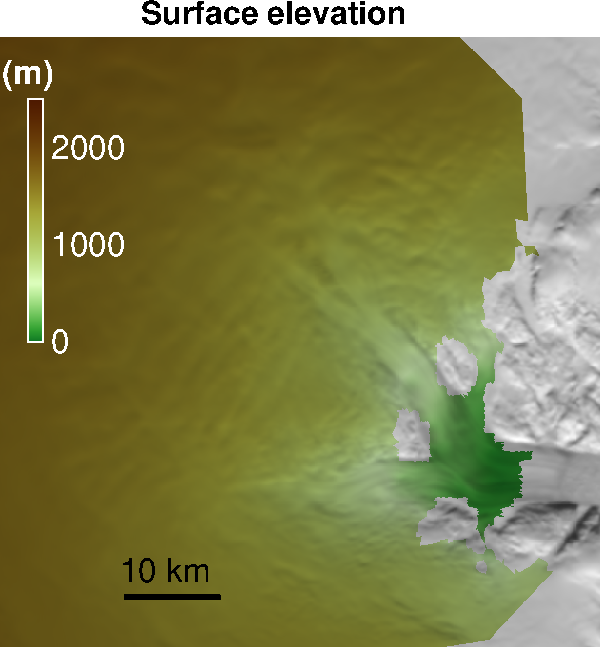
\includegraphics[width=0.21\textwidth]{subfigures/surface.pdf}};
    \node[empty] (fig3) at ($(SD3ll)!0.5!(Dtr)+(0, 0.05*\ly)$)
	 {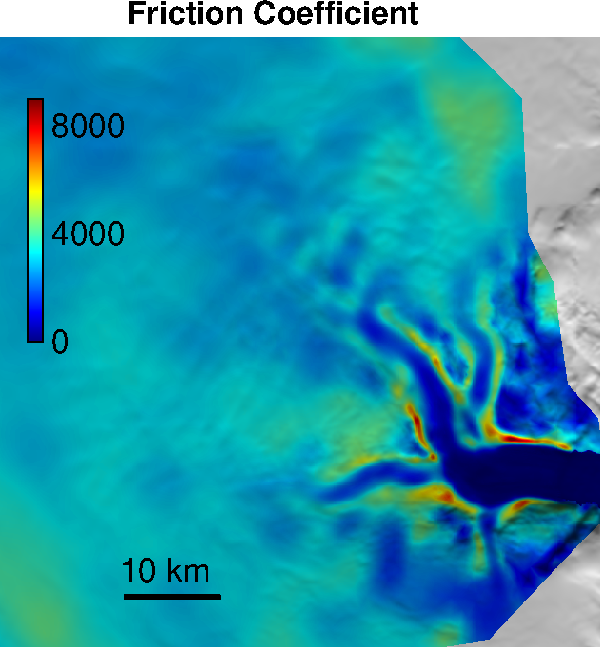
\includegraphics[width=0.21\textwidth]{subfigures/frictionC.pdf}};
    % Equations
    \normalsize
    \node[empty, scale=0.7] at ($(SD1ll)!0.5!(SD1tr)+(0.015*\lx, -0.14*\ly)$)
	 {$\mathcal{L}_u=w_{{u}} \|\boldsymbol{u}-\boldsymbol{u}^{\text{obs}}\|^2_{\boldsymbol{u}}$};
    \small
    \node[empty, scale=0.7] at ($(SD2ll)!0.5!(SD2tr)+(0, -0.14*\ly)$) {$\mathcal{L}_g=w_{{g}}\left(
	 \|{s}-{s}^{\text{obs}}\|^2_{{s}}+\|{H}-{H}^{\text{obs}}\|^2_{{H}}\right)$};
    \normalsize
    \node[empty, scale=0.7] at ($(SD3ll)!0.5!(Dtr)+(0, -0.14*\ly)$) {$\mathcal{L}_C=w_{C}
	 \|C-C^{\text{obs}}\|^2_{C}$};
    % arrows
    \draw[arrow, color=NavyBlue!90!white, to path={|- (\tikztotarget)}] ($(Lossmath)+(-0.065*\lx,0)$) --  +(0,-0.24*\ly) -| ($(fig1)+(0,0.14*\ly)$);
    \draw[arrow, color=NavyBlue!60!white, to path={|- (\tikztotarget)}] ($(Lossmath)+(0*\lx,0)$) --  +(0,-0.255*\ly) -| ($(fig2)+(0,0.14*\ly)$); 
    \draw[arrow, color=NavyBlue!30!white, to path={|- (\tikztotarget)}] ($(Lossmath)+(0.055*\lx,0)$) --  +(0,-0.27*\ly) -| ($(fig3)+(0,0.14*\ly)$);
    % text
	 \Large
    \node[empty, color=NavyBlue,rotate=90] (SDtext) at ($(fig1)+(-0.13*\lx,0)$) {Data};

    % ============================== Physics ==============================
    \draw[PBox] (Pll) rectangle (Ptr);
	 \normalsize
    % Equations
    \node[empty, scale=0.7] (SSA) at ($(Pll)!0.5!(Ptr)+(0,0.1*\ly)$) {$
    \begin{cases}
        \begin{aligned}
            \nabla\cdot\boldsymbol{\varsigma}+\boldsymbol{\tau}_b=\rho_i g H \nabla s, \quad \text{in } \Omega\\
            \boldsymbol{n}\cdot\boldsymbol{\varsigma}=(\bar{p}_i-\bar{p}_w)\boldsymbol{n} \quad \text{on } \Gamma
            \end{aligned}
    \end{cases}
    $};
    \node[empty, scale=0.8] at  ($(Pll)!0.5!(Ptr)+(0,-0.1*\ly)$) {$\mathcal{L}_f=w_{\Omega}\mathcal{L}_\Omega+w_{\Gamma}\mathcal{L}_\Gamma$};

    % arrow
    \draw[arrow, color=Orange!30!white, to path={|- (\tikztotarget)}] ($(Lossmath)+(0.12*\lx,0)$) --  +(0,-0.25*\ly) -| ($(Pll)!0.5!(Ptr)+(0,0.19*\ly)$);
    % text
	 \Large
    \node[empty, color=Orange] (Ptext) at ($(Pll)!0.5!(Ptr)+(0, -0.18*\ly)$) {Physics};

\end{tikzpicture}

\end{center}


\end{document}}
